
%include diagram

High energy electrons\footnote{Throughout this section we use 
electrons to collectively refer to both electrons and positrons
unless otherwise specified.} produced from the 
hard scatter of the proton-proton
collisions of the LHC
will frequently radiate photons in the presence of the ATLAS
detector material. Furthermore, it is also common %how common?
for high energy photons to decay into an electron-positron pair.
These two processes are shown as Feynman diagrams 
separately in \fig\ref{}.
Chaining these two processes together will cause 
an electron (positron) to radiate a photon which then produces an
electron-positron pair, resulting in a three body final state with
two electrons (positrons) and a positron (electron).
Often, the energy difference between the products in the final state will
be large, such that most of the energy is carried away in only one
product.  It is thus possible that majority of the energy of the initial
electron (positron) is carried away in the positron (electron), which
has an opposite charge.  If the energy imbalance is large enough,
the other two final state electrons (positrons) may not have enough
energy to be reconstructed. As a result, the initial electron
(positron) will instead be measured as a positron (electron), and the 
charge of initial state electron (positron) will have effectively 
been mis-identified. 


%need to do some research on Bethe-Bloche.
The probability of this to occur is non-negligible in the presence of the material 
from the ATLAS detector. This is due to bremstraahlung...
Look in 'experimental foundations' and in 'particle detection'


While muons are also technically also capable of such a phenomenon, the 
energies required are too large, according to Bethe-Bloche.
Indeed, we observe that the rate of charge mis-identification for muons
is vanishingly small and so we neglect it. %or should I just say that it should be?

The strong dependence of charge mis-identification 
upon the ATLAS material means that care must be
taken when describing this process. In particular, the material 
description in MC, while sophisticated, is not perfect. Thus, the use of MC
for determining the rate of electron charge mis-identification is inherently
flawed. Instead, it would be better to use the data itself to determine
a model for these rates. 
Thus, we extract the rates of electron charge 
mis-identification using the data and only use the rates determined
in MC as a cross-check.

The background due to electron charge mis-identification is most important 
for this analysis
in the 0 SFOS signal region, described in \sec\ref{sec:signal_regions},
where it is one of the only mechanisms by which the $WZ$ and $ZZ$ 
processes enter this region\footnote{The $WZ$ and $ZZ$ processes
can also enter in the 0 SFOS region if the $Z$ bosons
decay to $\tau$ leptons which then subsequently decay into 
either electrons or muons with the proper charge and flavor combination.}.
Without electron charge mis-identification, these events would fall
equally in the 1 and 2 SFOS regions.
As will be seen shortly, the overall rate of electron charge mis-identification
is quite small (calculate???). 
Furthermore, it will be seen that the total background in the 0 SFOS region is 
a good deal smaller than the 1 and 2 SFOS regions. Thus, the
migration of events from the 1 and 2 SFOS regions to the 0 SFOS 
region, resulting from electron charge mis-identification, has
a larger relative impact on the background in the 0 SFOS 
region\footnote{There is also a migration from the 0 SFOS to the 1 and 2 SFOS 
regions, but the relative number of 0 SFOS events to 1 and 2 SFOS
events before electron mis-identification is so small as to make this
effect completely negligible.}.
As a result, we focus only on modeling the background due to electron
charge mis-identification in the 0 SFOS region and assume that an 
out of the box estimate of this background from MC is adequate for the 
1 and 2 SFOS regions.


The electron charge mis-identification background is determined
for the 0 SFOS signal region by first extracting the electron charge
mis-identification rates using the data as a model,
described below. The extracted
rates are compared to an alternative method using only MC. 
The difference between the two is used as a systematic on the
rates. The rates are then used to re-weight the $WZ$ and $ZZ$ MC samples
on an event-by-event basis 
according to the probability that electron charge mis-identification
could cause the event to migrate into the 0 SFOS region. In this way, 
the full statistics of the MC samples can be utilized to get a model of
the behavior of these processes in the 0 SFOS region, while also taking 
into account a more accurate material description. Other backgrounds
due to electron charge mis-identification are assumed to be negligible.
More details on the methods used to extract the rates and the re-weighting
method are provided below.




\subsubsection{Charge Mis-identification Rate Extraction}

The rate of electron charge mis-identification is defined as 
the probability that an electron has its charge mis-identified.
These rates depend highly on the kinematics of the individual electrons.
In particular, the sensitivity to material dependence described above 
means that the rate depends on where in the detector the electrons
pass through. In general, the material density of the ATLAS
detector increases for high \eta~(i.e. as the electron gets closer to the
beam pipe), as seen in \sec\ref{sec:atlas_id}. The rate also increases as a function of the electron energy, 
or \pt. These are the two most important kinematic variables for determining
the rate\footnote{The material also varies as a function of the azimuthal angle,
$\phi$, in the detector. However, this is a sub-dominant effect. Furthermore,
increasing the dimensionality further significantly harms the statistical 
power of the method. Thus it is ignored.}, and 
so the rate extraction is binned as a function of both with nine $\eta$ 
bins ranging from 0 to 2.5 and six \pt~bins ranging from 15 to 120 \GeV~plus
an additional overflow bin for $\pt>120\GeV$.



The rates are studied in a region with two electrons passing the object
selection from \sec\ref{sec:object_selection} and that have
a di-lepton mass within 10~\GeV~of the \z~mass. No requirements are placed
on their charge. Two different methods
are used: one using purely MC and one using the data.
The method using MC takes $\z\rightarrow ee$ MC simulation 
and relies on being able to determine the charge of each electron from the 
\z~decay by looking 
directly at the hard scattering process as provided by the generator.
This is called ``truth'' information, at which point the processes of radiation
and pair-production have not occurred. It then compares
these truth electrons to the ``reconstructed'' electrons 
measured after all processes, including those of radiation and pair-production,
have been simulated and reconstructed
in the detector. The truth and reconstructed electrons
are matched by asking that they are nearby each other in $\eta$ and $\phi$.
The charge of the matched truth and reconstruction electrons 
are then compared to see if 
the charges agree
and tallying  this 
for the appropriate $\pt$ and $\eta$ bin. Once all MC events
have been recorded, the rate per bin may be determined simply 
by taking the ratio of the number of electrons where the truth and reconstructed
electron charge disagreed per bin to the total number of electrons per bin. 

The method using the data instead is the nominal method used 
for extracting the electron charge mis-identification
rates.
It uses the same selection as in the MC method, with the events
categorized based on whether the electrons from the \z~decay 
are of the same-sign or of opposite-sign.
However, in this case
there is no truth information to tell which electron's charge
has been mis-identified. Instead, we assume that those events in
the same-sign category are due purely to charge mis-identification
and attempt to extract the rates by minimizing a likelihood.
Refer to the rate for an electron in a 
particular $\pt$ and $\eta$ bin $i$ as $\varepsilon_i$.
Also, refer to the total number of di-electron events observed in data with one electron
in bin $i$ and the other in bin $j$ as $N_{i,j}$.
Given the rates, the expected number of same-sign events
should be approximately $N_{i,j}(\varepsilon_i + \varepsilon_j)$,
where we have ignored higher order terms, which account for  
the probability for both electrons to have their
charges flipped, since they should be small. We do
not know the rates \emph{a priori}, but they should follow 
a Poisson likelihood given the observed total number of events,
$N_{i,j}$, and the the observed number of same sign events,
$N_{i,j}^{\textrm{SS}}$, with the following form:
\begin{equation}
\curlyl( \varepsilon_i,\varepsilon_j | N_{i,j}^{\textrm{SS}},N_{i,j})
=
\frac{(N_{i,j}(\varepsilon_i+\varepsilon_j))^{N^{\textrm{SS}}_{i,j}} e^{-N_{i,j}(\varepsilon_i+\varepsilon_j)}}{N^{\textrm{SS}}_{i,j}!}
\end{equation}
From this, we may construct a log likelihood which can be minimized
as a function of $\varepsilon_i$ and $\varepsilon_j$:
\begin{equation}
-\ln \curlyl( \varepsilon_i,\varepsilon_j | N_{i,j}^{\textrm{SS}},N_{i,j}) = 
N_{i,j}(\varepsilon_i+\varepsilon_j)
- N^{\textrm{SS}}_{i,j} \ln(N_{i,j}(\varepsilon_i+\varepsilon_j))
\end{equation}
where the terms that are not dependent on $\varepsilon_i$
and $\varepsilon_j$ have been dropped.
Thus, given the data, the values of $\varepsilon_i$ and $\varepsilon_j$
at the minimum value of the log likelihood are taken as the estimate
of the rates.
We attempt to subtract backgrounds to the $Z\rightarrow ee$ process using a method described later.

\begin{figure}[htp]
\centering
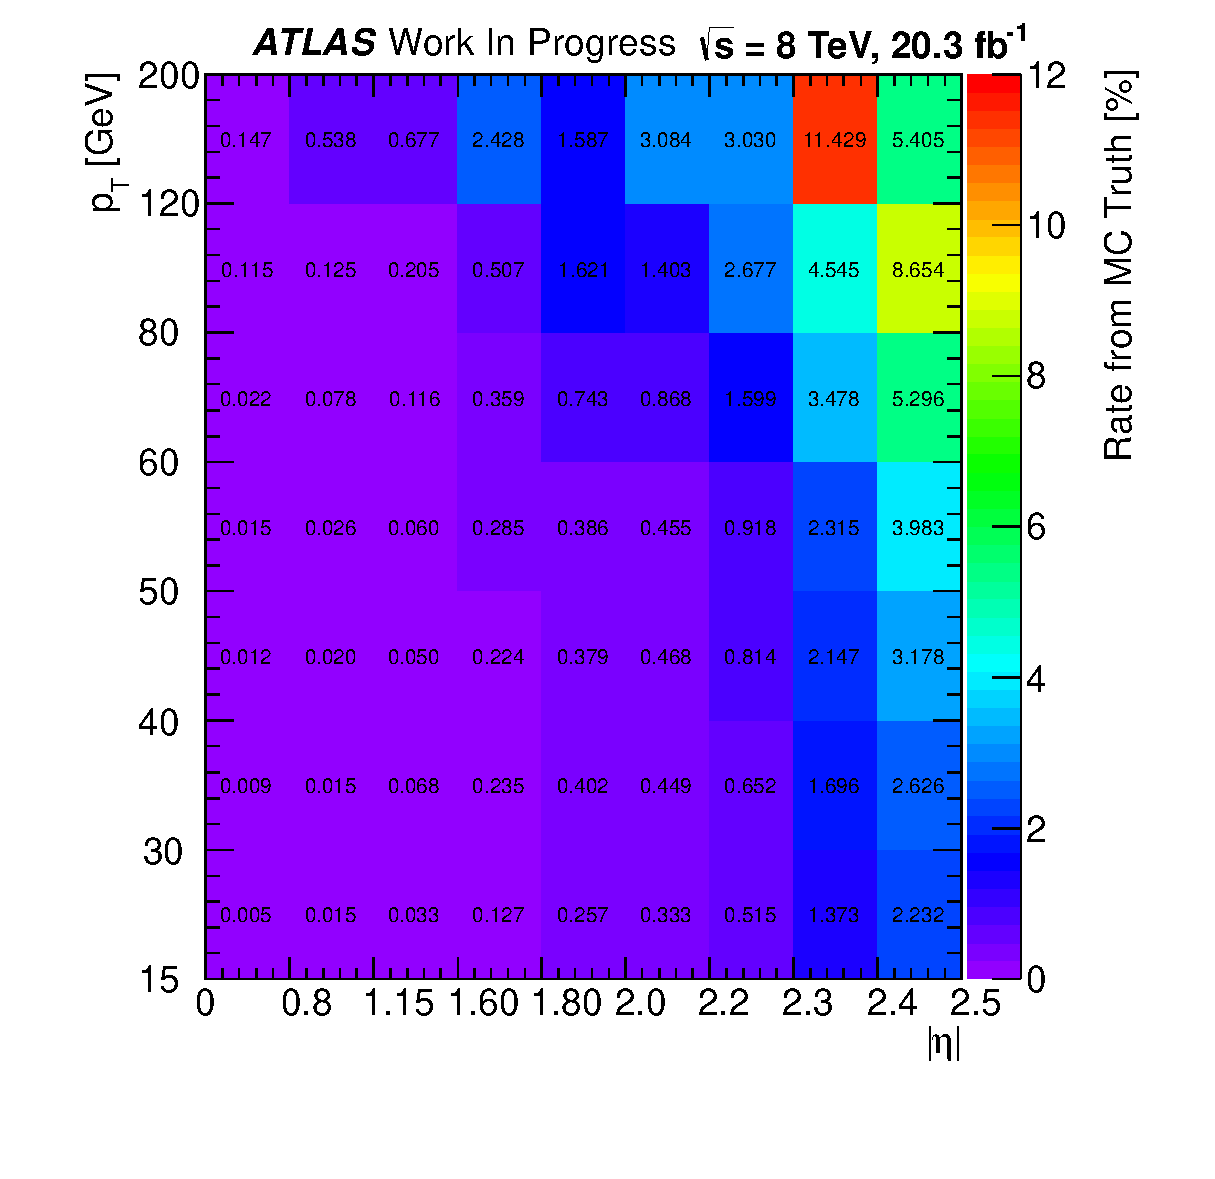
\includegraphics[width=0.45\columnwidth]{figures/ChargeMisID/Nov5_2015_TruthRates_Plot.eps}
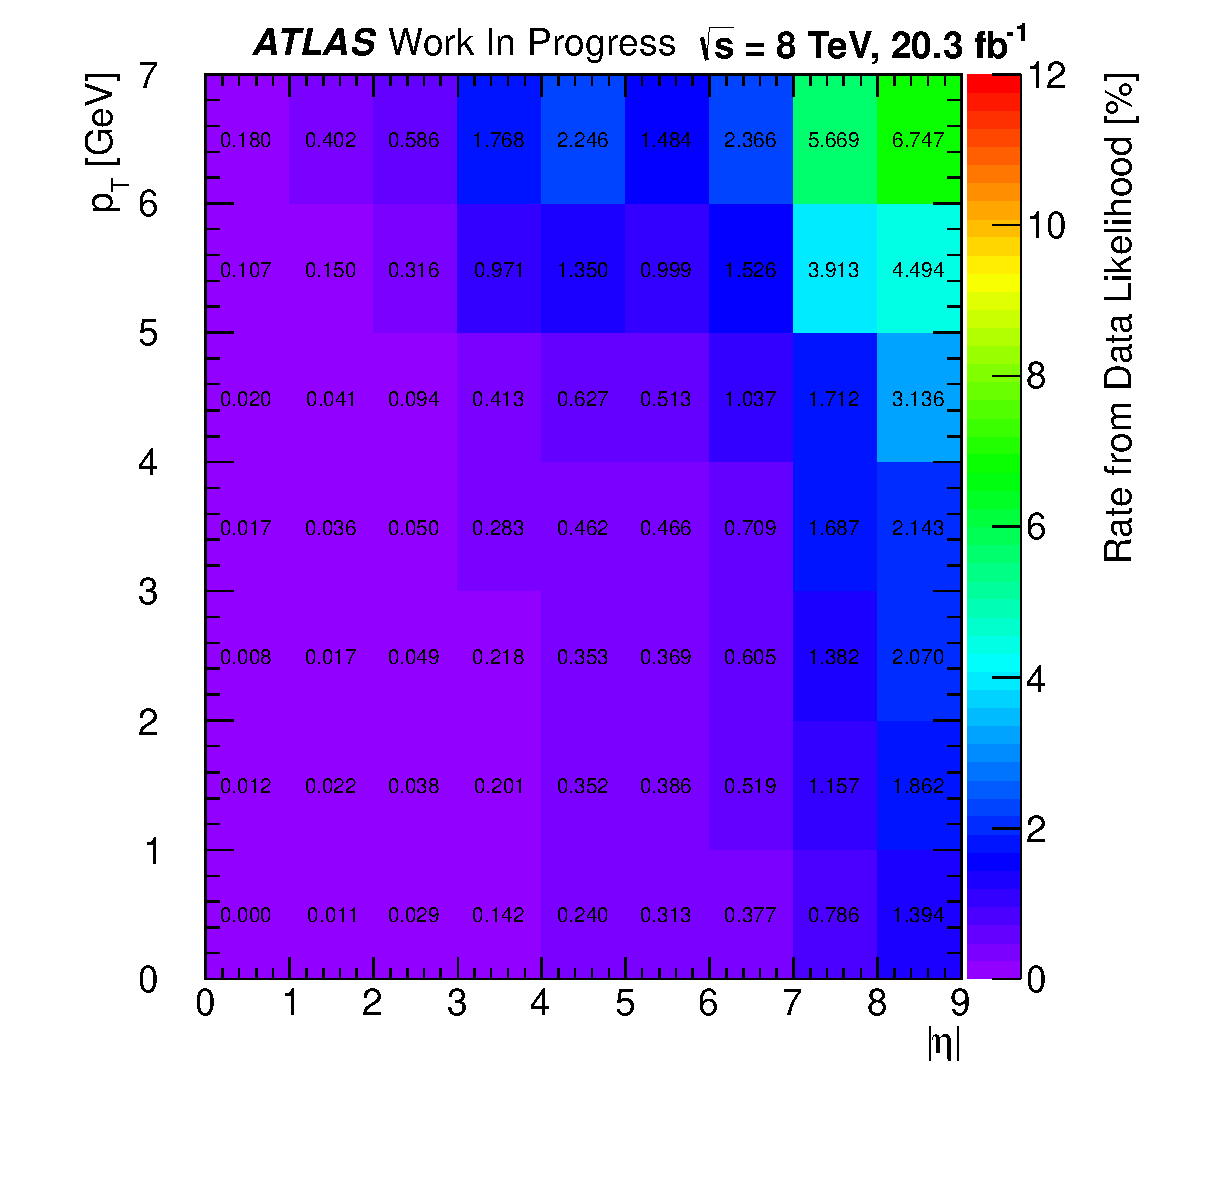
\includegraphics[width=0.45\columnwidth]{figures/ChargeMisID/Nov5_2015_DataRates_Plot.eps}
\caption{Electron charge mis-identification rates as a function of
the electron \pt and $\eta$ extracted using the MC
truth method (left) and the likelihood method in data (right). }
\label{fig:chargemisid_rates_contour}
\end{figure}

The rates for the two different methods are 
shown in \fig\ref{fig:chargemisid_rates_contour}.
For low values of \pt~and $\eta$, the rate is small enough to be negligible. 
The rate increases gradually along both dimensions, reaching as much as
6.7\% in the region $\pt > 120\GeV$ and $2.4 < |\eta| < 2.5$ as measured
in the data, which corresponds to the highest bin in both dimensions. 
The rates measured using MC truth information are systematically higher
than those measured in data, almost by a factor of two. The MC simulation
tends to overestimate the amount of material (figure?) actually in the
detector, which could explain this difference....
%figure 4.45 in jinst?
%or maybe https://atlas.web.cern.ch/Atlas/GROUPS/PHYSICS/PAPERS/PERF-2013-05/
%or https://atlas.web.cern.ch/Atlas/GROUPS/PHYSICS/PAPERS/PERF-2013-03/
%might it be that the material description was improved in a later version of the MC?
%mc12b is known to have a maybe 20-30% lower rate of photon conversions overall
%according to Jake, I guess because of the material description.
%could the improved simulation referred to in one of the papers above
%be for something that was included after mc12b? probably
%ruiqi used this sample for the MC generation:
%mc12 8TeV.147806.Powheg Pythia8 AU2CT10 Zee.merge.NTUP COMMON.e1169 s1469 s1470 r3542 r3549 p1562
%this twiki
%https://twiki.cern.ch/twiki/bin/view/Atlas/MC12cWiki?rev=3
%claims that improvements to the geometry came in mc12c
%However, these improvements claim that the improved geometry
%describes more material at high eta. It seems like this would only 
%make the disagreement between the mc and data rates, assuming
%that more material really does cause more conversion
%the paper claims the difference is in part to an incomplete
%description of SCT cooling pipes.
%the most discrepant region is between eta of 1.4 and 1.6, where the 
%difference would be consistent if material were removed.
%but this then would seem to suggest that the differences show up mostly
%in eta bin 3, which they do not. Instead it grows starting
%for eta > 2.0




%note: the material description shouldn't be affecting our zgamma
%estimate since it requires a b-layer hit so these are converting early

Some variations on the method are also performed
in order to better assess its performance 
and to determine systematic uncertainties.
One variation is to perform the same likelihood extraction
as in the data, but using only reconstructed MC. This produces
similar rates to the truth MC method, suggesting that the differences
seen between the data likelihood method and the truth MC method
are not due to the method itself. 
Another variation is to extract the rates from the data with the 
likelihood method but without performing the background
subtraction mentioned earlier. In the original method, 
the background subtraction is performed by... 
...with a template fit like in \fig\ref{fig:chargemisid_fitexample}.

\begin{figure}[htp]
\centering
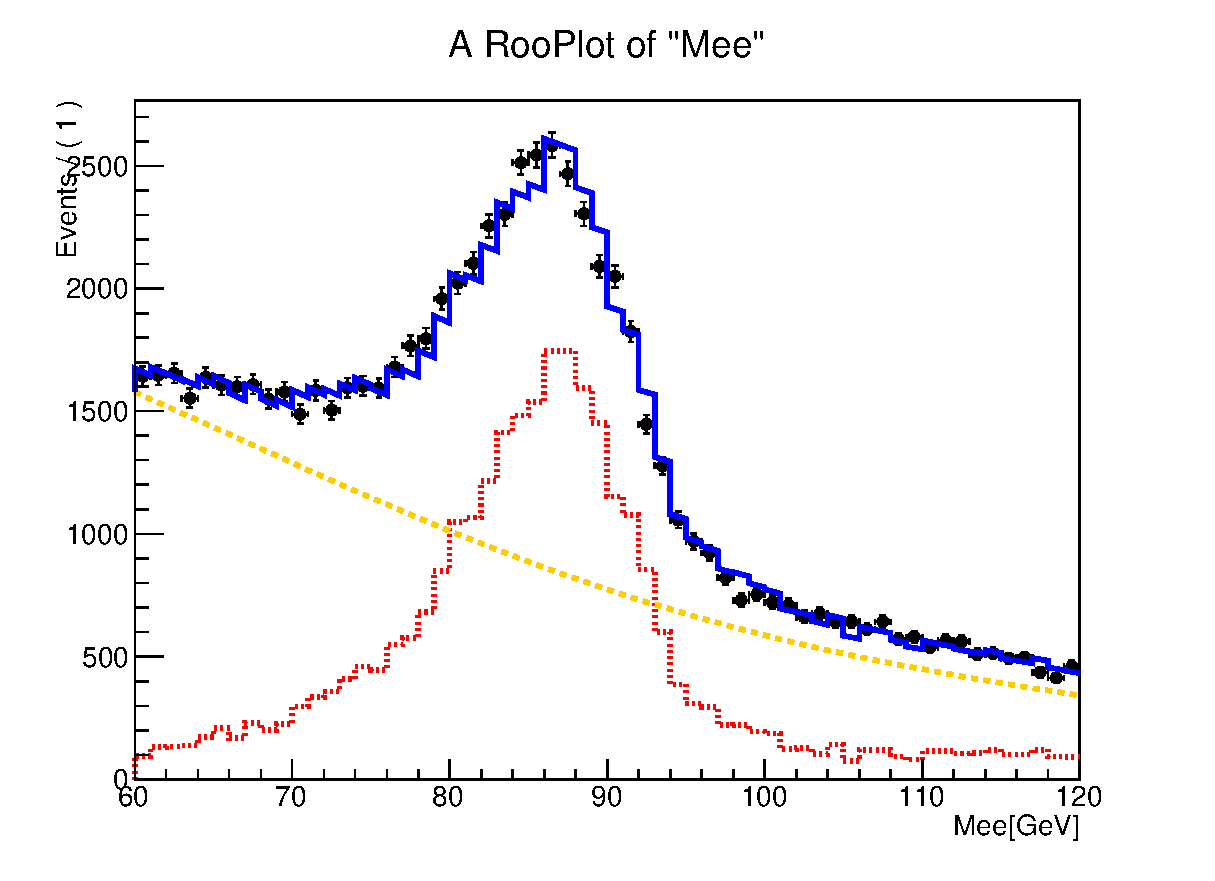
\includegraphics[width=0.6\textwidth]{figures/ChargeMisID/Tot_Polynomial_0_2.eps}
\caption{Plot of the di-lepton invariant mass 
in the region where one electron has $0 < |\eta_1| < 0.8$
and the other has $1.15 < |\eta_2|<1.6$. The data (black points)
are shown in a region where the electron isolation cuts are removed
and the electron quality requirements are loosened.
A template from $Z\rightarrow ee$ MC (red line) and a polynomial
curve (orange line) are used to fit the data. The sum of the fit
(blue line) is seen to fit the data well.}
\label{fig:chargemisid_fitexample}
\end{figure} 


The different variations on  rate estimation are compared to the 
nominal estimate to extract
a final systematic. In \fig\ref{fig:ChargeMisID_truthRate_finalFig},
the two-dimensional rates are unfolded into one-dimension
with the bins numbered counting from low values of $\eta$ and \pt~to
high values. The rates with and without background
subtraction are seen to agree quite well, only 
differing by about 5-6\% throughout.  
The MC truth method tends
to be larger than the rates in data by about a factor of two,
as was already mentioned. Finally, 
the red curve shows the rates evaluated using the same likelihood method
applied to the data, but using only reconstructed MC. 
Finally, the variation on the likelihood method using just MC
is seen to follow the MC truth method closely, except in a few bins where the statistics
are low. The relative difference between the MC truth and MC likelihood methods
is transported to the nominal estimate in data and used as another systematic.
The difference between the methods using data and those using MC is not
used as a systematic since such a difference is expected.
The systematic uncertainties are combined in quadrature with the statistical
uncertainty on the nominal estimate to arrive at a final uncertainty on the
rates, shown as a hashed band.


\begin{figure}[htp]
\centering
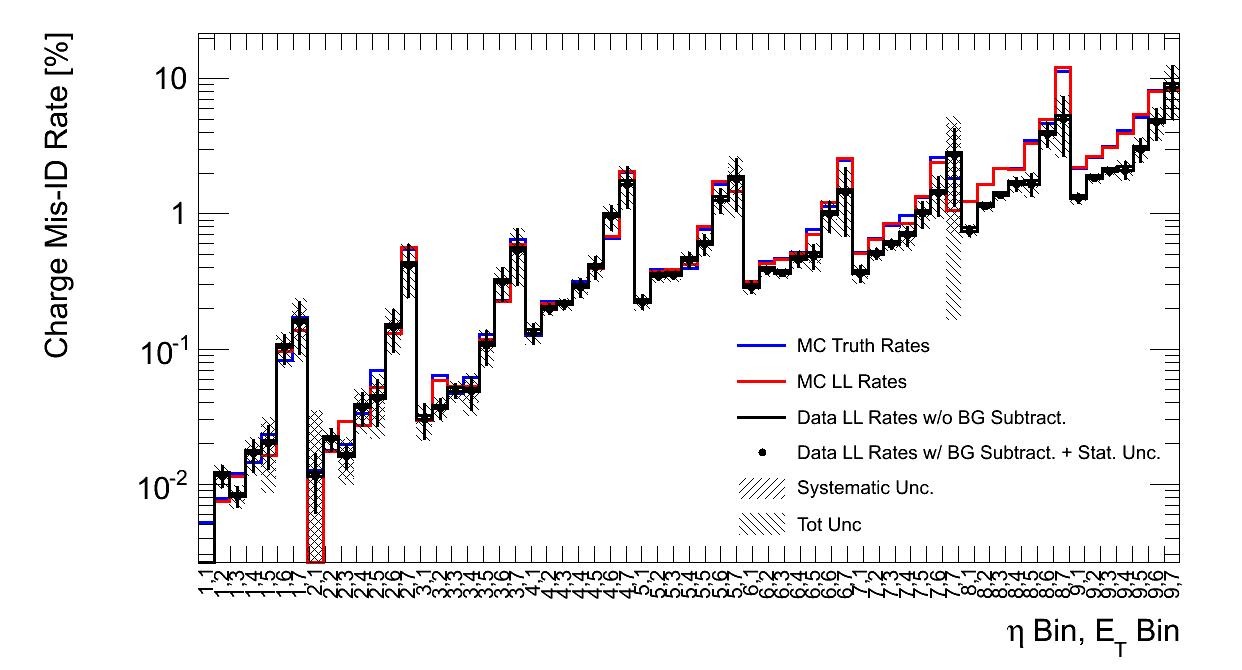
\includegraphics[width=0.9\textwidth]{figures/ChargeMisID/Validation_ChargeMisIDRates_PTvsEta_FinalRateWithSys.png}
\caption{Summary of electron charge mis-identification rates using
the likelihood method in data with background subtraction (black points) 
and without background subtraction (black line), the MC truth 
method (blue line), and the likelihood method in MC (red).
Systematic uncertainties are extracted as described in the text and are shown
in the gray hashed band pointing from bottom left to top right. 
The systematic uncertainties are combined with the statistical uncertainties
on the black points to arrive at a total uncertainty on the rates, shown 
in the hashed band pointing from bottom right to top left.}
\label{fig:ChargeMisID_truthRate_finalFig}
\end{figure}




\subsubsection{Di-boson MC Re-weighting}


The electron charge mis-identification  rates are primarily important for the determination of the $WZ$ and $ZZ$ background contamination in the 0 SFOS region,
as mentioned already.
Once derived, the rates are applied to $WZ$ and $ZZ$ MC samples based on 
whether or not a charge flip could cause the event to appear in the 0 SFOS region.  
In particular, the following di-boson decays are considered:
\begin{itemize}
\item $WZ\rightarrow e^{\pm}\nu~ e^{+}e^{-}$
\item $WZ\rightarrow \mu^{\pm}\nu~ e^{+}e^{-}$
\item $WZ\rightarrow \tau^{\pm}\nu~ e^{+}e^{-}$
\item $ZZ\rightarrow e^{+}e^{-}~e^{+}e^{-}$
\item $ZZ\rightarrow \mu^{+}\mu^{-}~ e^{+}e^{-}$
\end{itemize}
No other decay channels are considered.  These all share in common that they 
have at least one electron-positron pair.  
Except for the $WZ\rightarrow \tau^{\pm}\nu~e^{+}e^{-}$ decay channel, 
decay channels with tau leptons are not considered
because they are suppressed by the tau branching fraction and are 
thus negligible.

The charge mis-identification rates are then applied to these channels on an 
event-by-event basis as follows.
For each event that is processed, its decay channel is identified 
at truth level. Each reconstructed lepton
is examined  and assigned a rate, i.e. a probability to charge flip, 
based on its reconstructed $\pt$ and $\eta$ values.
The probability for a charge flip to occur in an event is then approximately 
the sum of rates for the individual electrons:
\begin{equation}
p(\textrm{Charge Mis-Identification in Event}) \approx \sum_{i \in \textrm{Electrons}}  \textrm{Rate}(\pt^i,\eta^i) 
\end{equation}
Higher order terms where multiple electrons are charge mis-identified is negligible.
We are only concerned with the probability that a charge flip results in the 
event falling into the 0 SFOS region. 
Consider a step function, $\Theta(e)$, defined for an individual event:
\[
\Theta(e) = 
\begin{cases}
\hfill 1 \hfill & \text{if flipping charge of $e$ classifies event as 0 SFOS} \\
\hfill 0 \hfill & \text{if flipping charge of $e$ does NOT classify event as 0 SFOS}\\
\end{cases}
\]
Then the probability that a charge mis-identification occurs and results in 
the event falling in the 0 SFOS region is:
\begin{equation}
p(\textrm{Event is classified as 0 SFOS}) \approx \sum_{i \in \textrm{Electrons}}  \textrm{Rate}(\pt^i,\eta^i)\Theta(i) 
\end{equation}
Again, we ignore the case where multiple electrons have their charge 
mis-identified.  This probability is then used as an event-by-event weight. 


Once the weight has been determined, we then artificially flip the charge of 
one of the electrons/positrons in the event.
If there is only one electron in the event that will lead the event 
to fall in the 0 SFOS region, its charge is flipped
and one proceeds to the next event.  However, if there are multiple electrons 
in the event, there is an ambiguity that must be resolved
about which electron's charge should be flipped. One must then be careful in 
this case to not introduce any bias.
We decided to choose a procedure where we pick a single electron from the 
event at random based on the charge flip rates
of the individual electrons. Thus, for an individual electron in an 
event, the probability that it is chosen to have its charge
flipped is:
\begin{equation}
p(\textrm{$e$ has been charge flipped}) = \textrm{Rate}(\pt^e,\eta^e)\Theta(e)~/\sum_{i \in \textrm{Electrons}} \textrm{Rate}(\pt^i,\eta^i)\Theta(i)
\end{equation}

Consider an example where the event under consideration comes from the 
decay $WZ\rightarrow e^{+}\nu e^{+}e^{-}$. Assume all three charged leptons 
pass reconstruction and are selected then label 
them as: $e^{+}_1~e^{+}_2e^{-}_3$. In this case,
the only way that this event could be classified as 0 SFOS when 
flipping the charge of only one electron/positron is to flip the 
charge of the electron.
Thus, $\Theta(e^{+}_1)=\Theta(e^{+}_2)=0$ and $\Theta(e^{-}_3)=1$.  The event 
weight will then be equal to the rate of charge mis-identification 
for  $e^{-}_3$ and it will have it's charge flipped 
to be positive\footnote{This results in a final state
which does not fall into our signal region, since the sum of the
charge of the three electrons is +3. Thus, it is just for illustration purposes}.

Now consider an example of an event with 
the decay of $ZZ\rightarrow \mu^{+}\mu^{-}~ e^{+}e^{-}$.
If all four leptons are reconstructed and selected, the event will not 
be considered at all in the three lepton selection of this analysis, so 
consider the case where the $\mu^{+}$ is not selected leaving three leptons 
labeled as: $\mu^{-}_1 e^{+}_2 e^{-}_3$.  The probability for the muon to 
charge flip is negligible which leaves the electron and the positron. Flipping 
the charge of either one at a time will result in the event being 
classified as 0 SFOS.  Thus, in
this case $\Theta(\mu^{-}_1)=0$ and $\Theta(e^{+}_2)=\Theta(e^{-}_3)=1$. The 
event weight will then be the sum of the rates for $e^{+}_2$ and $e^{-}_3$.
The probability that the electron has its charge flipped is then 
$\frac{\textrm{Rate}(e^{-}_3) }{ \textrm{Rate}(e^{+}_2)+ \textrm{Rate}(e^{-}_3)}$ 
and similarly for the positron.

\subsubsection{Validation}
This procedure has been validated on the $WZ$ and $ZZ$ samples by comparing 
the predictions taken directly from MC to the predictions re-weighted in the 
0 SFOS signal region using the procedure just described. This is done in 
\fig\ref{fig:ChargeMisID_Validation_WZ} for the $WZ$ samples and on 
\fig\ref{fig:ChargeMisID_Validation_ZZ} for the $ZZ$ samples. It can be seen 
the agreement in the shape looks good for all the distributions. An offset 
between the two distributions is observed. This difference is covered partially by 
the systematic uncertainties of the method.  Any remaining difference could 
be expected from the difference in rates observed at high $\eta$ and 
high $E_{T}$ as seen in Fig.~\ref{fig:ChargeMisID_truthRate_finalFig} and 
serves as justification for using the data-driven method.

There is no special treatment of the charge mis-identification contribution to 
other background contributions in the 0 SFOS region or to any contributions to the 
1 and 2 SFOS signal regions, including di-boson processes, as the effect is 
expected to be very small.  Any charge mis-identification events are thus 
taken directly from MC in this case.


 \begin{figure}[htp]
 \centering
 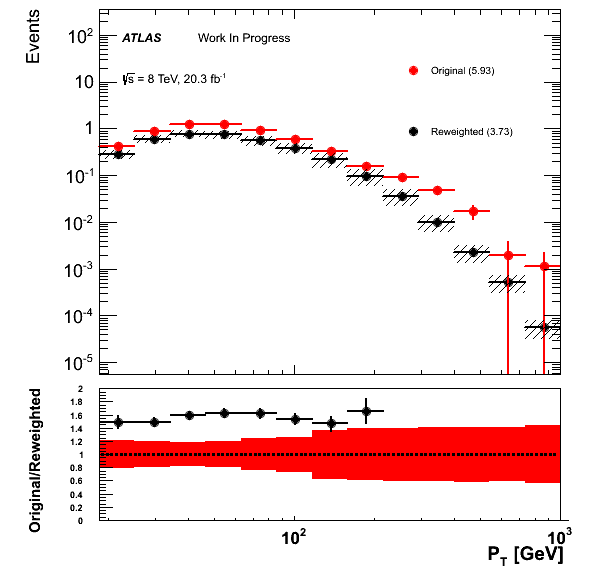
\includegraphics[width=0.4\textwidth]{figures/ChargeMisID/Validation_ChargeMisIDRates_WZ_PTLepton.png}
 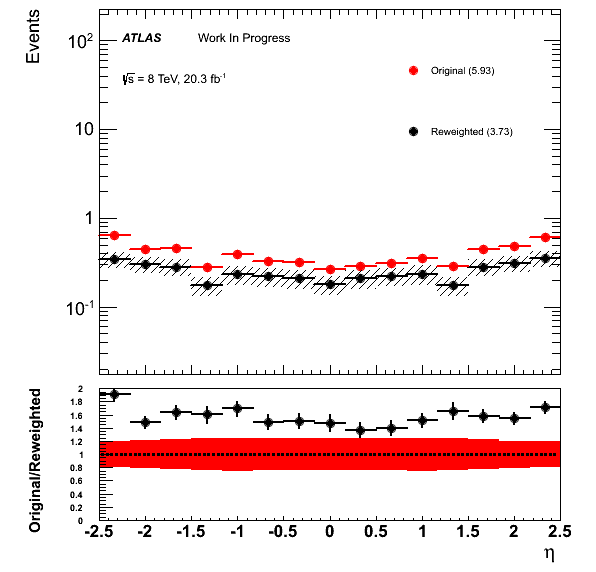
\includegraphics[width=0.4\textwidth]{figures/ChargeMisID/Validation_ChargeMisIDRates_WZ_EtaLepton.png}
 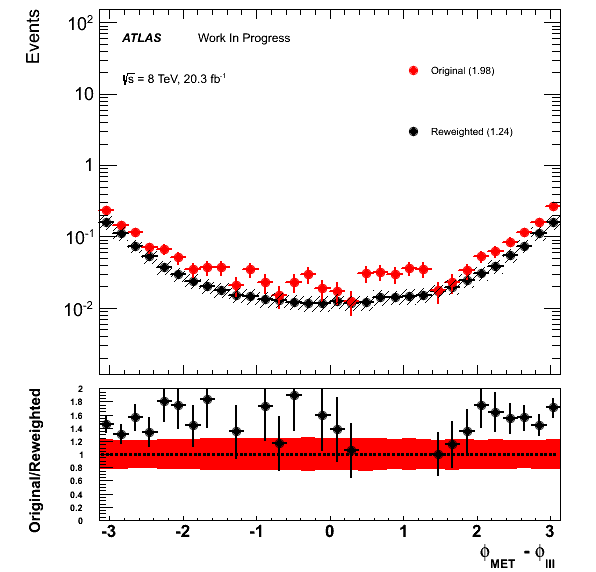
\includegraphics[width=0.4\textwidth]{figures/ChargeMisID/Validation_ChargeMisIDRates_WZ_DeltaPhi.png}
 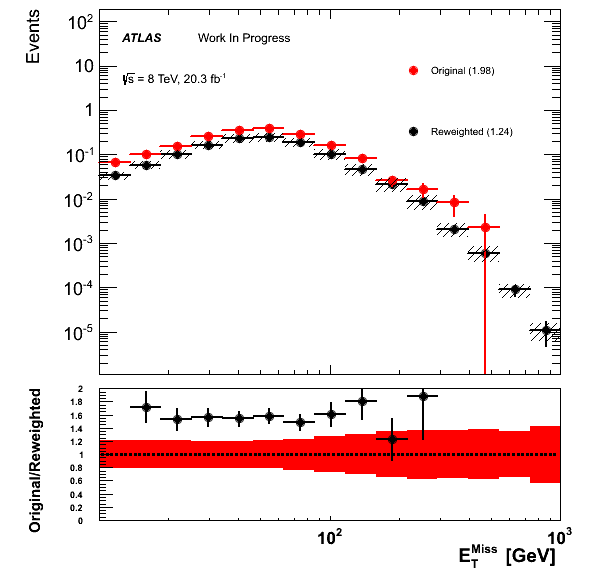
\includegraphics[width=0.4\textwidth]{figures/ChargeMisID/Validation_ChargeMisIDRates_WZ_MET.png}
 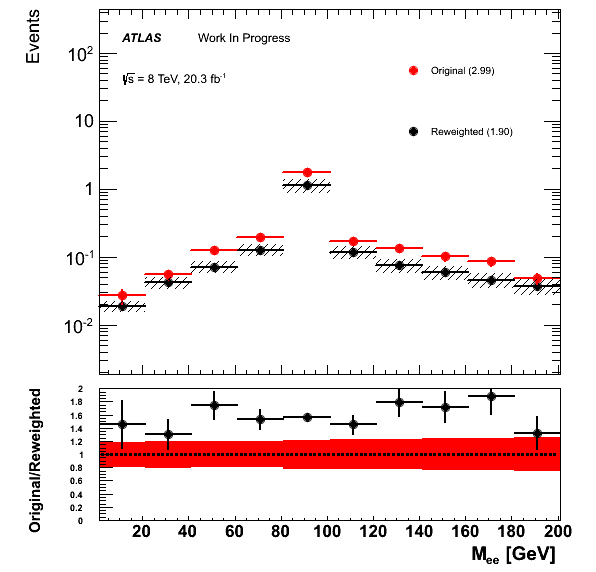
\includegraphics[width=0.4\textwidth]{figures/ChargeMisID/Validation_ChargeMisIDRates_WZ_Mee.png}
 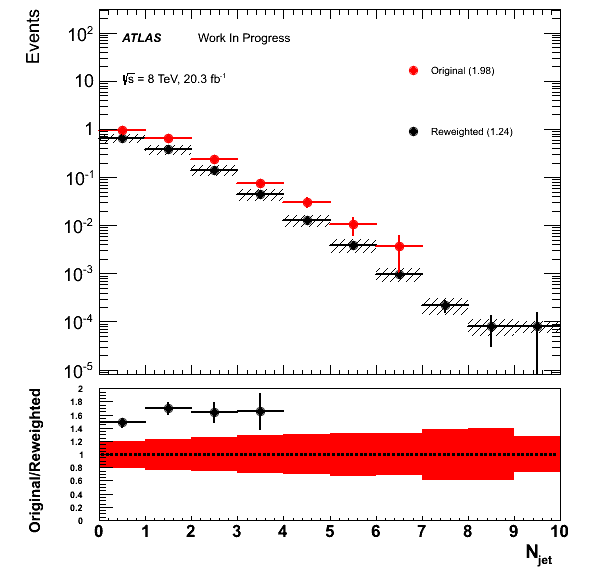
\includegraphics[width=0.4\textwidth]{figures/ChargeMisID/Validation_ChargeMisIDRates_WZ_JetMultiplicity.png}

 \caption{Validation of the charge mis-ID rates comparing 
 MC $WZ\rightarrow \ell ee$ ($\ell=e,\mu$) samples re-weighted with the 
 charge mis-ID rates measured in the MC $Z\to{}ee$ 
 sample to the original MC predictions. Distribution of 
 lepton $p_{T}$, $\eta$, $\Delta \phi(3l,E_{T}^{Miss})$,\met{}, Same-sign 
 di-electron invariant mass, and jet multiplicity.}
 \label{fig:ChargeMisID_Validation_WZ}
 \end{figure}
 
 
 \begin{figure}[htp]
 \centering
 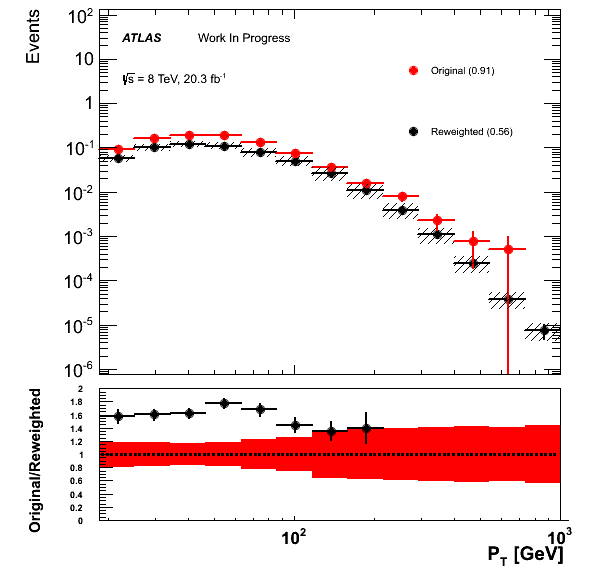
\includegraphics[width=0.4\textwidth]{figures/ChargeMisID/Validation_ChargeMisIDRates_ZZ_PTLepton.png}
 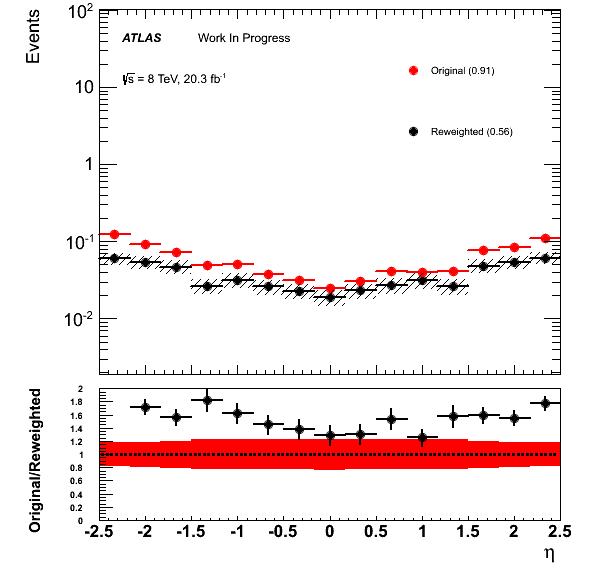
\includegraphics[width=0.4\textwidth]{figures/ChargeMisID/Validation_ChargeMisIDRates_ZZ_EtaLepton.png}
 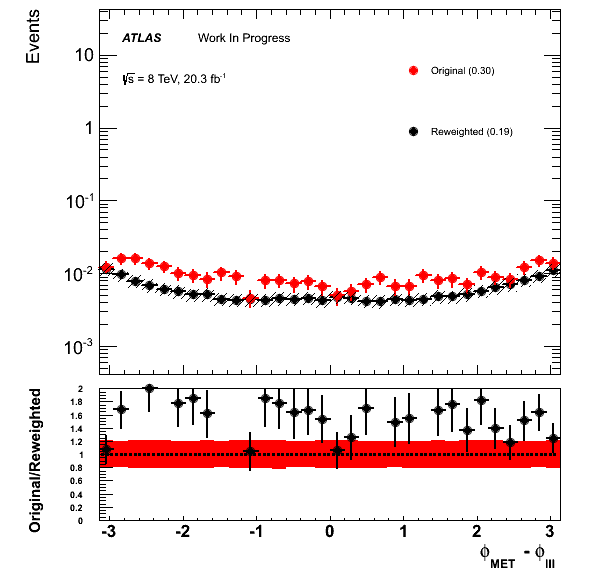
\includegraphics[width=0.4\textwidth]{figures/ChargeMisID/Validation_ChargeMisIDRates_ZZ_DeltaPhi.png}
 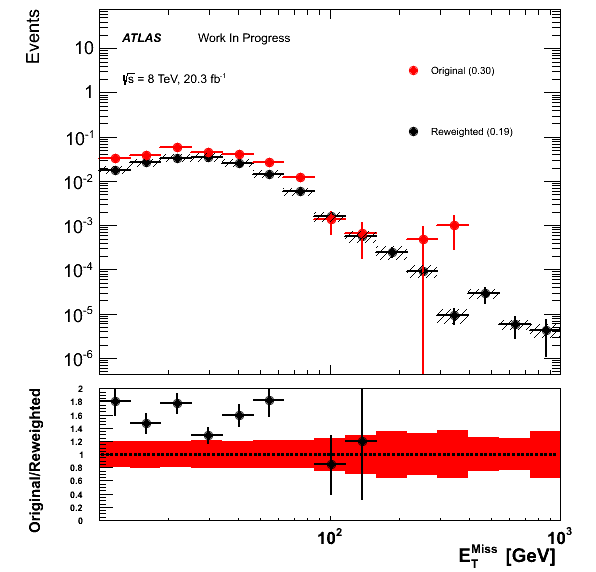
\includegraphics[width=0.4\textwidth]{figures/ChargeMisID/Validation_ChargeMisIDRates_ZZ_MET.png}
 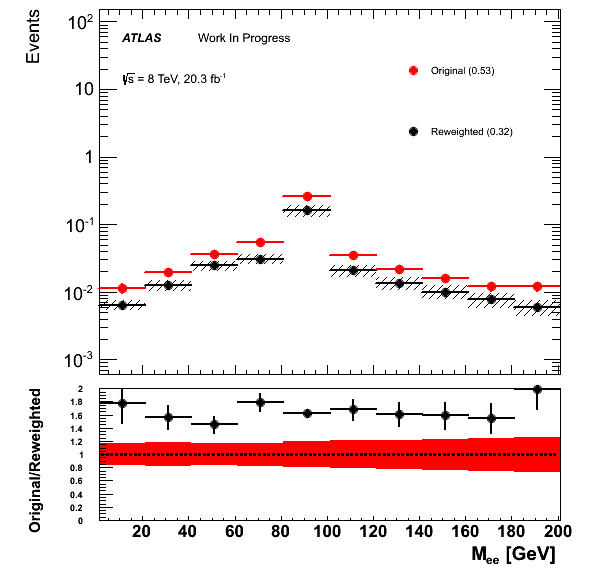
\includegraphics[width=0.4\textwidth]{figures/ChargeMisID/Validation_ChargeMisIDRates_ZZ_Mee.png}
 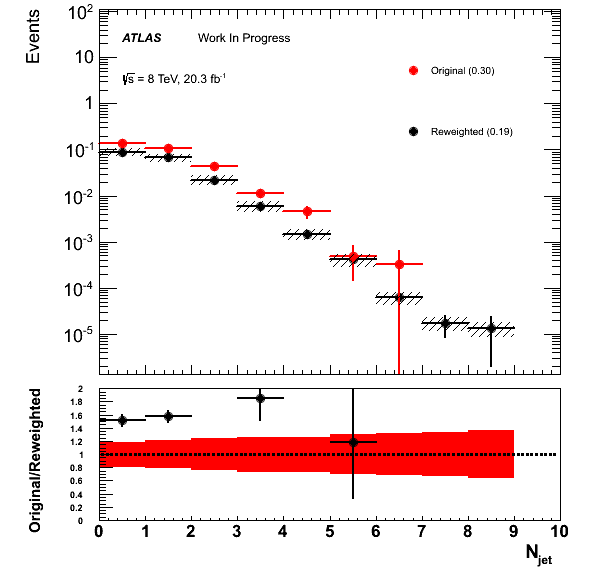
\includegraphics[width=0.4\textwidth]{figures/ChargeMisID/Validation_ChargeMisIDRates_ZZ_JetMultiplicity.png}

 \caption{Validation of the charge mis-ID rates comparing 
 MC $ZZ\rightarrow \ell \ell ee$ ($\ell=e,\mu$) samples re-weighted with the 
 charge mis-ID rates measured in the MC $Z\to{}ee$ 
 sample to the original MC predictions. Distribution of 
 lepton $p_{T}$, $\eta$, $\Delta \phi(3l,E_{T}^{Miss})$,\met{}, Same-sign 
 di-electron invariant mass, and jet multiplicity.}
 \label{fig:ChargeMisID_Validation_ZZ}
 \end{figure}



